\documentclass[a4paper]{article}
\usepackage[14pt]{extsizes}
\usepackage[T2A]{fontenc}
\usepackage[utf8]{inputenc}
\usepackage[english, russian]{babel}
\usepackage{geometry}
\geometry{left=2cm}
\geometry{right=1.5cm}
\geometry{top=1.5cm}
\geometry{bottom=1.5cm}
\usepackage{hyperref}
\usepackage{graphicx} 
\usepackage{tabto}
\usepackage{setspace}
\usepackage{color} 
\usepackage{listings}
\usepackage{algorithm}
\usepackage{algpseudocode}
\lstset{
extendedchars= \true
}

\begin{document}
\begin{onehalfspacing}
\begin{titlepage}
	\begin{center}
		{Федеральное агенство связи \\ Федеральное государственное бюджетное образовательное учреждение высшего образования "Сибирский государственный университет телекоммуникаций и информатики"\\[5pt]}
		\vspace{1.5cm}
		\begin{flushright}
			{\normalsize\bfseries Кафедра ТСиВС}\\
		\end{flushright}
		\vspace{2cm}
		{\Large Отчет по курсовой работе\\по дисциплине: <<Моделирование распределенных систем>>\\на тему: <<Моделирование движения абонентов по дорогам>> } \\[2cm]
		\begin{flushleft}
			{\tab Выполнили:\\\tab студенки группы ИА-831:\\\tab Когустова Влада Васильевна\\\tab Угольникова Екатерина Алексеевна} \\[1cm]
			{\tab Проверили:\\\tab доцент кафедры ТСиВС\\\tab Дроздова Вера Геннадьевна\\\tab ведущий инженер кафедры ТСиВС\\\tab Ахпашев Руслан Владимирович}
		\end{flushleft}
		\vfill
		{Новосибирск 2020}
	\end{center}
	
\end{titlepage}   

%------------------------------------------------------------

\clearpage

\tableofcontents
\clearpage
\section{Задание курсовой работы}

\tab Требуется разработать web-страницу, отображающую карту местности. На карте необходимо случайным образом отрисовать базовые станции (BS) и абонентские устройства (UE). Базовые станции статичны. Абонентские устройства могут двигаться, могут стоять на месте.

План курсовой работы:
\begin{enumerate}
	\item Создать Web-страницу c картой (yandex || google || openstreetmap).

	\item Создать несколько абонентов (минимум 10) и отобразить их на карте (маркеры\textbackslash картинки\textbackslash схема).

	\item Абоненты должены двигаться только по дорогам (изменение координат абонентов относительно времени).

	\item Шаг изменения координат зависит от скорости абонента.

	\item 50\% абонентов должны ходить со скоростью от 3 до 7 км/ч, 50\% абонентов со скоростью от 30 до 70 км/ч.
\end{enumerate}


\section{Цель работы}

\tab Целью данной курсовой работы является знакомство с языком программирования javascript и использованием API для работы с разными картами (Google, Yandex). Реализация моделирования движения абонентов по карте, при ограничении области движения дорогами. 

\clearpage
\section{Ход работы}
\subsection*{Краткое описание алгоритма выполнения курсовой работы}

\tab Для начала мы инициализировали карту и создали необходимое количетсво абонентов со случайными координатами (они так же являются маркерами) и научили их ходить случайным образом по всей карте.

Потом мы добавили некоторые элементы управления и приступили к работе с API для получения необходимых данных с помощью get-запросов к сервисам Google и Yandex. 

С помощью сервиса Google Maps Roads API нам удается получить точку на ближайшей дороге, в которую перемещается маркер. Таким образом каждый маркер, созданный в случайном месте, перемещается на ближайшую дорогу. Далее для маркера находящегося на дороге, генерируется случайное место назначения, в которое должен переместиться маркер. С помощью get-запроса к Roads API  получаем обьект, сожержащий некоторое количество точек, которые представляют собой маршрут, по которому двигаются маркеры. 

После завершения движения по одному маршруту сразу же генерируется новый, начиная с точки в которой закончился предыдущий. Абоненты (маркеры) продолжают двигаться по своим маршрутам и создавать новые, до тех пор пока не будет нажата кнопка ''Stop Movement''.

Ознакомиться с готовым курсовым проектом можно перейдя по ссылке в приложении 1. Так же там представлена документация к  проекту, с которой можно ознакомится при необходимости.

\clearpage


\section{Результаты работы}
\begin{figure}[h!]
	\centering
	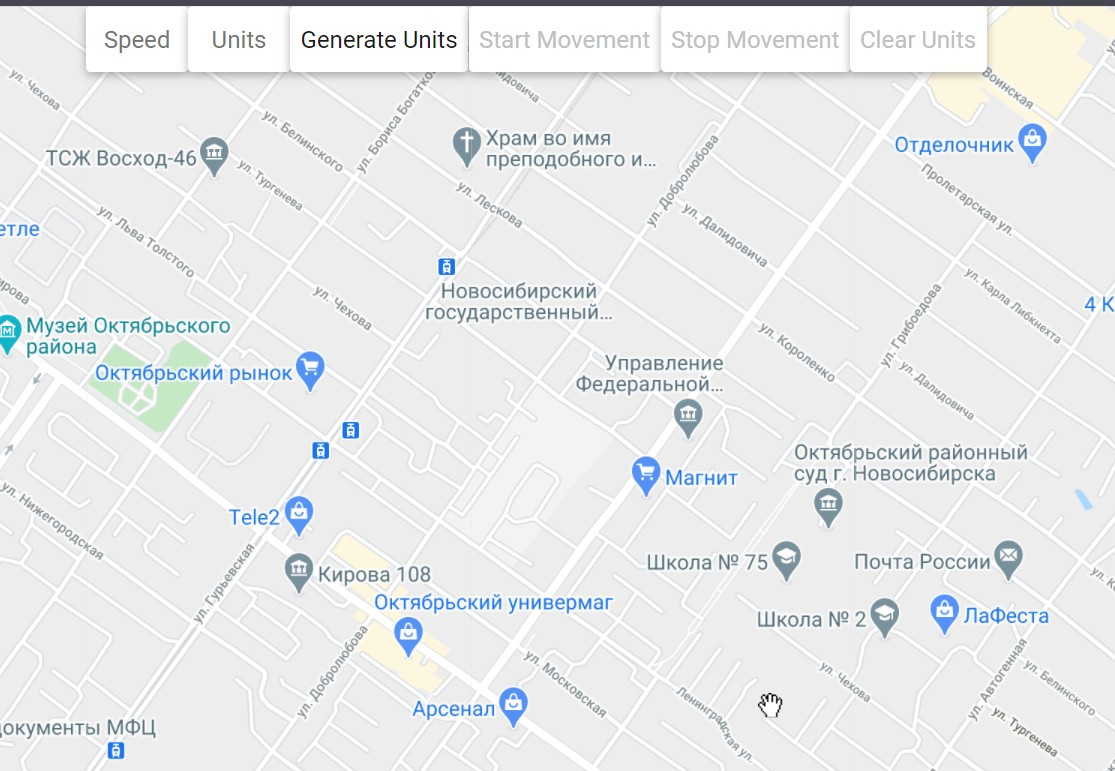
\includegraphics[width=0.8\linewidth]{C:/Users/vcogu/Desktop/JS_MRS-Kate/report/image/init_maps}
	\caption{Вид карты, при запуске}
	\label{fig:mpr}
\end{figure}
\begin{figure}[h!]
	\centering
	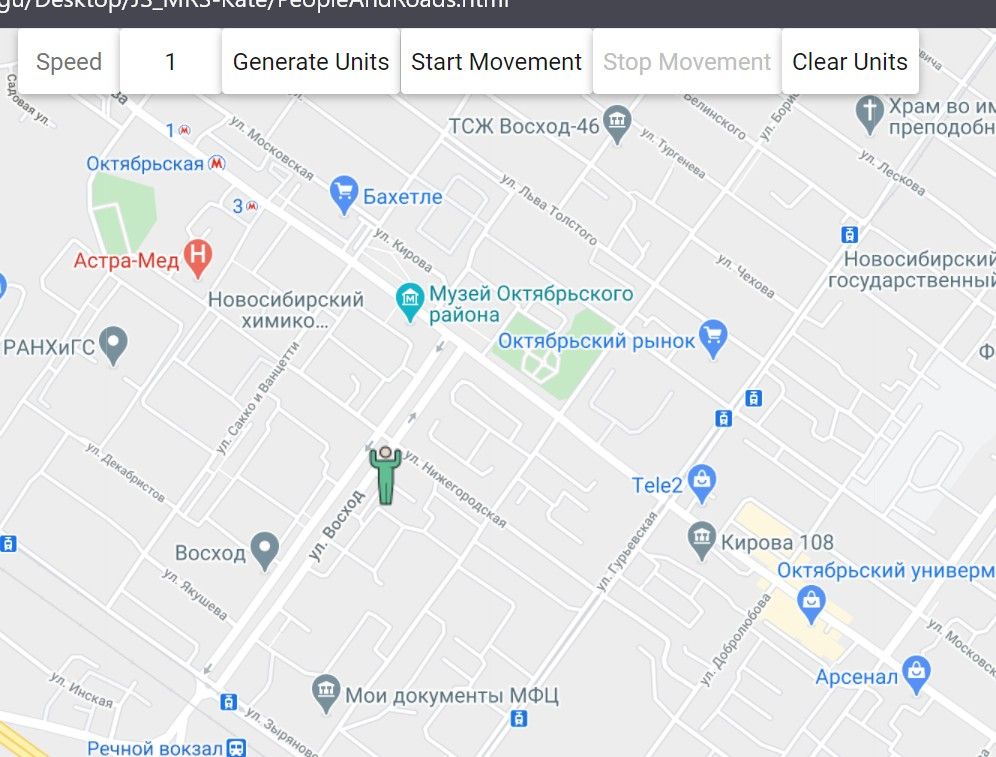
\includegraphics[width=0.8\linewidth]{C:/Users/vcogu/Desktop/JS_MRS-Kate/report/image/generation_1unit}
	\caption{Создание определенного количества абонентов}
	\label{fig:mpr}
\end{figure}
\begin{figure}[h!]
	\centering
	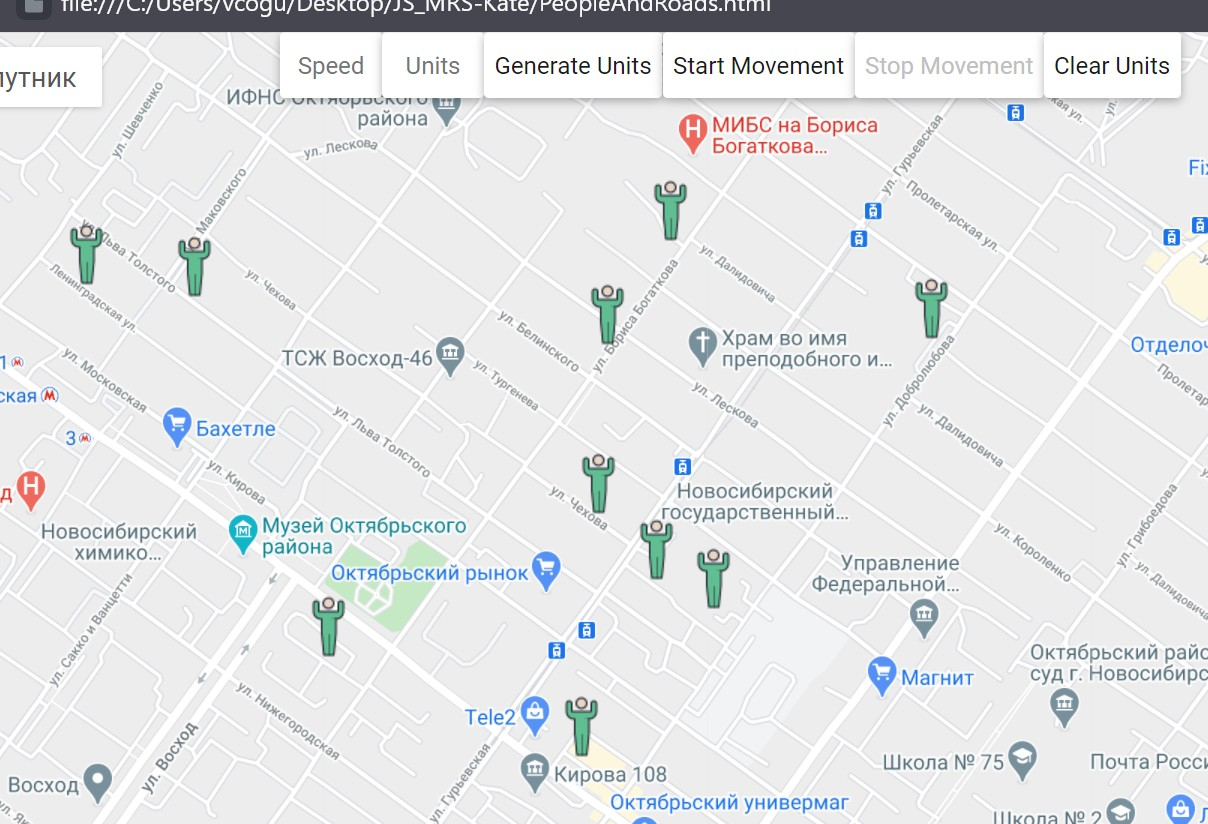
\includegraphics[width=0.8\linewidth]{C:/Users/vcogu/Desktop/JS_MRS-Kate/report/image/if_no_number_unit}
	\caption{Если не задать колличество абонентов, то создатся по умолчанию 10 абонентов }
	\label{fig:mpr}
\end{figure}
\begin{figure}[h!]
	\centering
	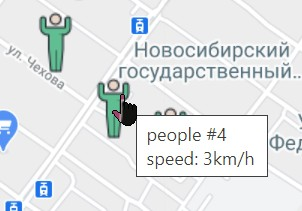
\includegraphics[width=0.8\linewidth]{C:/Users/vcogu/Desktop/JS_MRS-Kate/report/image/unit_4kmh}
	\caption{Скорость одного из абонентов }
	\label{fig:mpr}
\end{figure}
\begin{figure}[h!]
	\centering
	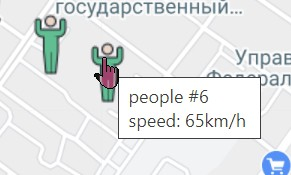
\includegraphics[width=0.9\linewidth]{C:/Users/vcogu/Desktop/JS_MRS-Kate/report/image/unit_65kmh}
	\caption{Скорость одного из абонентов }
	\label{fig:mpr}
\end{figure}
\begin{figure}[h!]
	\centering
	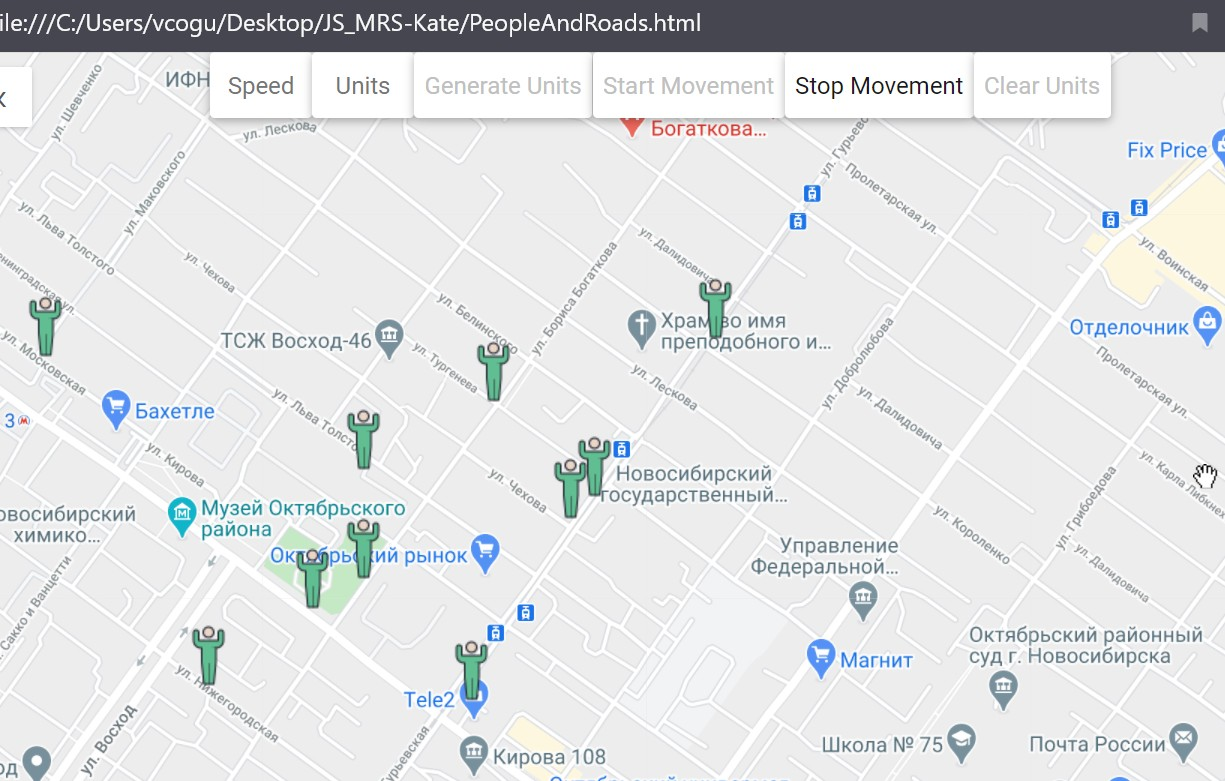
\includegraphics[width=0.9\linewidth]{C:/Users/vcogu/Desktop/JS_MRS-Kate/report/image/movement_unit}
	\caption{При движении абонентов, остальные кнопки блокируются, кроме Stop Movement }
	\label{fig:mpr}
\end{figure}
\begin{figure}[h!]
	\centering
	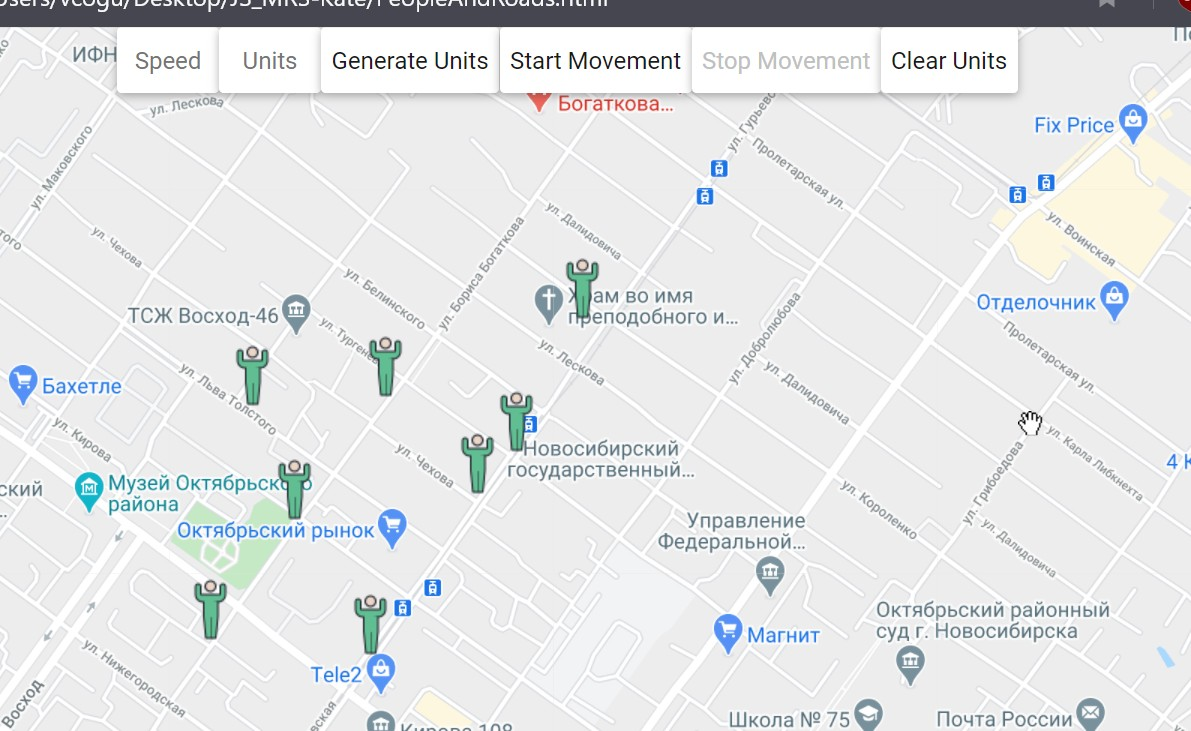
\includegraphics[width=0.9\linewidth]{C:/Users/vcogu/Desktop/JS_MRS-Kate/report/image/stop_movement}
	\caption{При остановке абонентов, остальные кнопки доступны, кроме Stop Movement }
	\label{fig:mpr}
\end{figure}
\begin{figure}[h!]
	\centering
	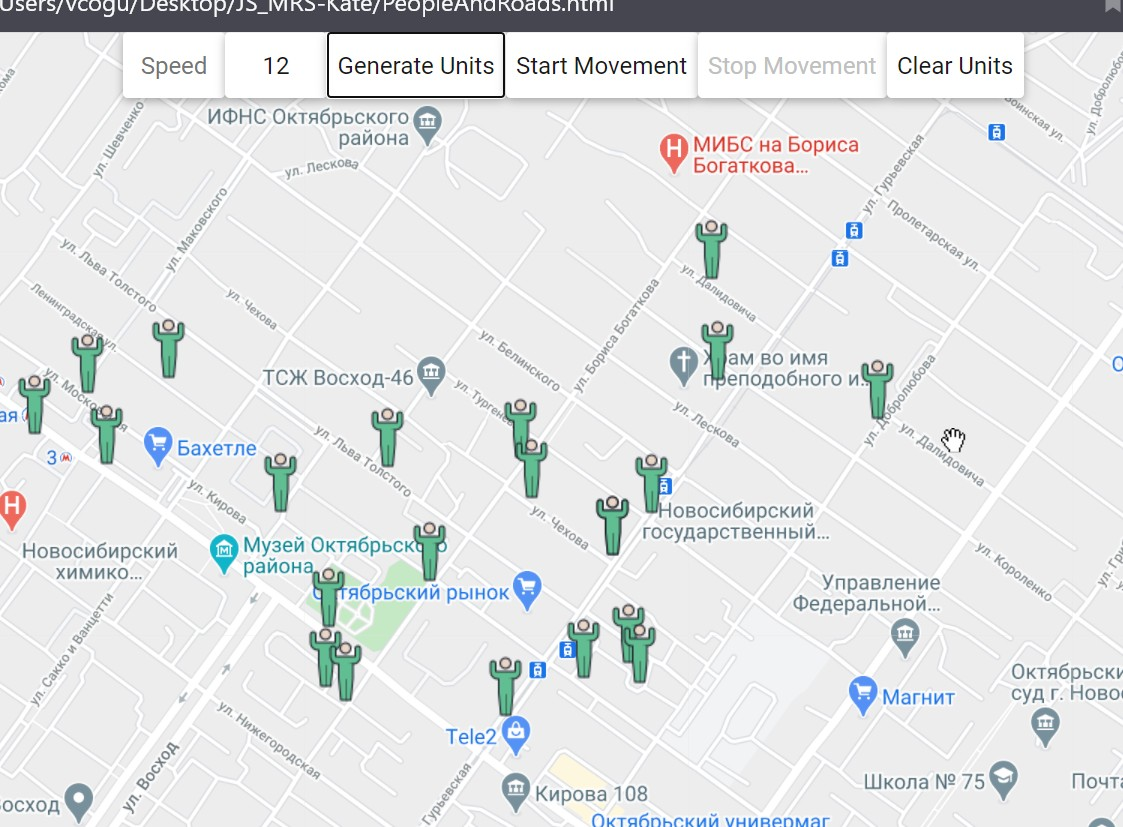
\includegraphics[width=0.9\linewidth]{C:/Users/vcogu/Desktop/JS_MRS-Kate/report/image/generate_new_unit}
	\caption{Создание новых дополнительных абонентов }
	\label{fig:mpr}
\end{figure}
\clearpage
\section{Вывод}

\tab В результате выполнения курсовой работы создана web-страница для взаимодействия с картами Google Maps. Реализовано моделирование движения абонентов по карте, при ограничении области движения дорогами.

Получены навыки работы с языком программирования javascript и стеком языков разметки html/css; навыки работы с картами и их API, навыки написания get-запросов и обработки ответов, представленных данными в JSON формате. 

В результате взаимодействия с сервисами предоставления API у разных вендоров (Gooble, Yamdex) получен незабываемый опыт несправедливого оценивания количества отправленных get-запросов со стороны Yamdex Maps API, впервые так сильно хотелось дождаться наступления нового дня по Московскому времени. А благодаря Gooble Maps API получен первый в жизни кредит, на целых 300\$!

\section*{Приложение 1}
\addcontentsline{toc}{section}{Приложение 1}

\begin{enumerate}

	\item \href {https://github.com/SLADKAY-KISA/JS_MRS.git}{Проект курсовой работы на платформе GitHub}.
	
\end{enumerate}
\end{onehalfspacing}

\clearpage
\section*{Приложение 2}
\addcontentsline{toc}{section}{Приложение 2}
\begin{lstlisting}[language=python,tabsize = 1,breaklines=true, breakatwhitespace=false,frame=single]
const Struct = (...keys) => ((...v) => keys.reduce((o, k, i) => {o[k] = v[i]; return o} , {}))
	const Item = Struct('marker', 'speed')
	const Step = Struct('step_lat', 'step_lng')
		
	let markers = [];
	var interval1;
	var flag = 0;
	var chicago = { lat: 55.014690, lng: 82.959608 };
		
	let NumberOfPointsAtRoad = [];
	var view_result = [];
	function randomInRange(min, max) {
	return Math.random() < 0.5 ? ((1-Math.random()) * (max-min) + min) : (Math.random() * (max-min) + min);
		} 

		/**
			 * 
			 * 
			 */
		function randomizeInteger(min, max) {
			if(max == null) {
				max = (min == null ? Number.MAX_SAFE_INTEGER : min);
			min = 0;
			}
			min = Math.ceil(min);  // inclusive min
			max = Math.floor(max); // exclusive max
			if(min > max - 1) {
				throw new Error("Incorrect arguments.");
			}
			return min + Math.floor((max - min) * Math.random());
		}

		function rad(x) {
			return x * Math.PI / 180;
		}
		function DistanceBetweenTwoPoints(point1_lat, point1_lng, point2_lat, point2_lng){
			//marker1, marker2) {
			var R = 6378137;
			var dLat = rad(point2_lat - point1_lat);
			var dLong = rad(point2_lng - point1_lng);
			var a = Math.sin(dLat / 2) * Math.sin(dLat / 2) + 
			Math.cos(rad(point1_lat)) * Math.cos(rad(point2_lat)) *
			Math.sin(dLong / 2) * Math.sin(dLong / 2);
			var c = 2 * Math.atan2(Math.sqrt(a), Math.sqrt(1 - a));
			var d = R * c;
			return d;
			// console.log(d);
		};
		function setNewPosition(marker, x, y){
			var latlng = new google.maps.LatLng(x, y);
			marker.setPosition(latlng);
		}

	   function getRoadsApi(x, y, option) {
		  
			x1 = randomInRange(55.021465, 55.012316);
			y1 = randomInRange(82.936089, 82.963985); 
			let URL_for_roads = "https://roads.googleapis.com/v1/snapToRoads?path=";
			let URL_x = x;
			let URL_y = y;
			let URL_x1 = x1;
			let URL_y1 = y1;
			let URL_interpolate = "&interpolate=true";
			let URL_key = "&key=YOUR_KEY";
			let URL_for_roads1 =  URL_for_roads.concat(URL_x,",",URL_y,"|",URL_x1,",",URL_y1,URL_interpolate,URL_key);
			var x_setNew_possion ;
			var y_setNew_possion ;
			var DATA;
					$.ajax({
						url: URL_for_roads1,
						method: "GET",
						async: false
					}).then(function(dataRoad) {
						console.log(dataRoad);
						x_setNew_possion = dataRoad.snappedPoints[0].location.latitude;
						y_setNew_possion = dataRoad.snappedPoints[0].location.longitude;
						DATA=dataRoad;
					});
			switch(option){
				case 1:
					return [x_setNew_possion,y_setNew_possion];
				case 2:
					return DATA;
			}				
		}

		function CreateUnits(map, Number, markers) {

			for (var j = markers.length, i = 0; i < Number; i++, j++) {
				let x;	
        		let y; 		
        		let speed;	
				var position;	
				var icon1 = 'https://img.icons8.com/plasticine/50/000000/arms-up.png';
				var icon2 = 'https://img.icons8.com/plasticine/60/000000/person-laying-down.png'
				x = randomInRange(55.021465, 55.012316); 
				y = randomInRange(82.936089, 82.963985); 
				var infoWindow;
				position = { lat: x, lng: y}; 
				if(i < Number/2) {
					speed =  randomizeInteger(3,7);
					
					var marker = new google.maps.Marker({
					position: position,
					map: map,
					//title: "people #"+j +" speed: " + speed + "km/h",
					icon: icon1,
					});
					var infoWindow = new google.maps.InfoWindow({
					content: speed + ' km/h',
					

					}); 
					 

					marker.addListener("mouseover", function(){ 

					infoWindow.open(map, marker);

					});

					marker.addListener('mouseout', function(){ 

					infoWindow.close()

					});

					}
				
				else{
					speed =  randomizeInteger(30,70);
					
					var marker = new google.maps.Marker({
					position: position,
					map: map,
					//title: "people #"+j+" speed: " + speed + "km/h",
					icon: icon1,
					});
					var infoWindow = new google.maps.InfoWindow({ 

					content: speed + ' km/h',
					//content: i + 'pepople'

					});

					

					marker.addListener('mouseout', function(){
					infoWindow.close()

					});

					}
				

				
				var positionAtRoad =  getRoadsApi(x, y, 1);
				var latlng = new google.maps.LatLng({lat: positionAtRoad[0], lng: positionAtRoad[1]});
				marker.setPosition(latlng);
				markers.push(Item(marker, speed));	
				view_result.push();
				NumberOfPointsAtRoad.push(0);

}
}

		function oneStep(markers,view_result, j, i){
				// console.log("I'm people #"+j+" and I'm walking "+i+" step!!");
				
				setNewPosition(markers[j].marker, view_result[j].snappedPoints[i-1].location.latitude, view_result[j].snappedPoints[i-1].location.longitude);
					//console.log("lat: "+markers[j].marker.getPosition().lat()+"lng: "+markers[j].marker.getPosition().lng());
				
		}

		function GenerateNewRoad(markers, j, view_result, NumberOfPointsAtRoad){
			view_result[j]=getRoadsApi(markers[j].marker.getPosition().lat(),markers[j].marker.getPosition().lng(), 2);
			//console.log("view_result["+j+"]: "+view_result[j]);
			NumberOfPointsAtRoad[j]=view_result[j].snappedPoints.length;
			console.log("view_result["+j+"].snapped: "+view_result[j].snappedPoints.length);
		}

		function UnitsMovement(map, Number, markers) {	
			for(var j = 0; j < Number; j++){
				console.log("Units Movement numb: "+Number);			
				console.log("Begin movement!!! unit: "+j+"      lat == "+markers[j].marker.getPosition().lat()+" lng == "+markers[j].marker.getPosition().lng());

				GenerateNewRoad(markers, j, view_result, NumberOfPointsAtRoad);
				//console.log("view_result["+j+"]: "+view_result[j]);
				//console.log("view_result["+j+"].snapped: "+view_result[j].snappedPoints.length);
			}

			var t=1;
			var tt = []; 
			currentstep = []; 
			for(var j = 0; j < Number; j++){
				tt.push(1);
				var diff = PointsDifference(
						markers[j].marker.getPosition().lat(),
						markers[j].marker.getPosition().lng(),
						view_result[j].snappedPoints[1].location.latitude,
						view_result[j].snappedPoints[1].location.longitude);
				var distance = DistanceBetweenTwoPoints(
						markers[j].marker.getPosition().lat(),
						markers[j].marker.getPosition().lng(),
						view_result[j].snappedPoints[1].location.latitude,
						view_result[j].snappedPoints[1].location.longitude);
				var beginstep = StepBetweenPoints(diff, markers[j].speed, distance);
				currentstep.push(Step(beginstep[0], beginstep[1]));
			}
			console.log(currentstep);

			interval2 = setInterval(function(){
				for(j = 0; j < Number; j++){
					if(flag == 1){ 
						clearInterval(interval2);
						flag = 0;
					}

					
					if(tt[j] == NumberOfPointsAtRoad[j]){ 
						GenerateNewRoad(markers, j, view_result, NumberOfPointsAtRoad);
						tt[j]=1; //
					}
					
					if( Math.abs(markers[j].marker.getPosition().lat() - view_result[j].snappedPoints[tt[j]].location.latitude) <= 0.00001 &&
						Math.abs(markers[j].marker.getPosition().lng() - view_result[j].snappedPoints[tt[j]].location.longitude) <= 0.00001){
						tt[j]++;
						
						var diff = PointsDifference(
							markers[j].marker.getPosition().lat(),
							markers[j].marker.getPosition().lng(),
							view_result[j].snappedPoints[tt[j]].location.latitude,
							view_result[j].snappedPoints[tt[j]].location.longitude);
						var distance = DistanceBetweenTwoPoints(
								markers[j].marker.getPosition().lat(),
								markers[j].marker.getPosition().lng(),
								view_result[j].snappedPoints[tt[j]].location.latitude,
								view_result[j].snappedPoints[tt[j]].location.longitude);
						var newstep = StepBetweenPoints(diff, markers[j].speed, distance);
						currentstep[j] = Step(newstep[0], newstep[1]);

					}
					
					else{
						setNewPosition(
							markers[j].marker, 
							markers[j].marker.getPosition().lat()+currentstep[j].step_lat, 
							markers[j].marker.getPosition().lng()+currentstep[j].step_lng
						);

					}
				}
				t++;
			}, 100);
		}

		function UI_ForButtons(controlUI){
			controlUI.style.backgroundColor = "#fff";
			controlUI.style.border = "2px solid #fff";
			controlUI.style.borderRadius = "3px";
			controlUI.style.boxShadow = "0 2px 6px rgba(0,0,0,.3)";
			controlUI.style.cursor = "pointer";

			controlUI.style.textAlign = "center";
			controlUI.style.color = "rgb(25,25,25)";
			controlUI.style.fontFamily = "Roboto,Arial,sans-serif";
			controlUI.style.fontSize = "16px";
			controlUI.style.lineHeight = "38px";
			controlUI.style.paddingLeft = "5px";
			controlUI.style.paddingRight = "5px";

		}

		 function GeneratePeople_Button(controlDiv, map, markers) {

			controlDiv.id = "Generate";
			UI_ForButtons(controlDiv);
			controlDiv.title = "Click to generate Units";
			controlDiv.innerHTML = "Generate Units";
			controlDiv.style.color = "rgb(25,25,25)";

			controlDiv.addEventListener("click", () => {
				var Number = 10;
				var numb = document.getElementById("Number");
				if(numb.value != 0)
					Number = numb.value;
				// console.log(numb.value);
				var button = document.getElementById("Start");
				button.removeAttribute("disabled");
				button.style.color = "rgb(25,25,25)";

				var button1 = document.getElementById("Clear");
				button1.removeAttribute("disabled");
				button1.style.color = "rgb(25,25,25)";
				CreateUnits(map, Number, markers);
						
			});
		}
	
		function StartMoving_Button(controlDiv, map, markers) {

			controlDiv.id = "Start";
			UI_ForButtons(controlDiv);
			controlDiv.title = "Click to start the Units movement";
			controlDiv.style.color = "rgb(192,192,192)";
			controlDiv.innerHTML = "Start Movement";

			controlDiv.addEventListener("click", () => {


				var Speed = 10;
				var Sp = document.getElementById("Speed");
				if(Sp.value != 0)
					Speed = Sp.value;
				// console.log(Sp.value);

				controlDiv.setAttribute("disabled", "");
				controlDiv.style.color = "rgb(192,192,192)";

				var button = document.getElementById("Generate");
				button.setAttribute("disabled", "");
				button.style.color = "rgb(192,192,192)";

				var button1 = document.getElementById("Clear");
				button1.setAttribute("disabled", "");
				button1.style.color = "rgb(192,192,192)";

				var button2 = document.getElementById("Stop");
				button2.removeAttribute("disabled");
				button2.style.color = "rgb(25,25,25)";

				var Number = markers.length;
				UnitsMovement(map, Number, markers);
			});
		}

		function StopMoving_Button(controlDiv, map, interval,markers){

			controlDiv.id = "Stop";
			UI_ForButtons(controlDiv);
			controlDiv.title = "Click to stop the Units movement";
			controlDiv.style.color = "rgb(192,192,192)";
			controlDiv.innerHTML = "Stop Movement";

			controlDiv.addEventListener("click", () => {

				controlDiv.setAttribute("disabled", "");
				controlDiv.style.color = "rgb(192,192,192)";

				var button = document.getElementById("Generate");
				button.removeAttribute("disabled");
				button.style.color = "rgb(25,25,25)";

				var button1 = document.getElementById("Clear");
				button1.removeAttribute("disabled");
				button1.style.color = "rgb(25,25,25)";

				var button2 = document.getElementById("Start");
				button2.removeAttribute("disabled");
				button2.style.color = "rgb(25,25,25)";


				var Number = markers.length;
				console.log("SUKA "+Number);
				console.log("ITS BEEN CLICKED: " + flag);
				for(var j = 0; j < Number; j++){
					console.log("ERTYUI "+j);
					console.log("End!!! unit: "+j+"      lat == "+markers[j].marker.getPosition().lat()+" lng == "+markers[j].marker.getPosition().lng());

				}

				flag = 1;
			});
		}

		function ClearUnits_Button(controlDiv, markers){

			controlDiv.id = "Clear";
			UI_ForButtons(controlDiv);
			controlDiv.title = "Click to clear the Units";
			controlDiv.innerHTML = "Clear Units";
			controlDiv.style.color = "rgb(192,192,192)";

			controlDiv.addEventListener("click", () => {

			controlDiv.setAttribute("disabled", "");
			controlDiv.style.color = "rgb(192,192,192)";

			
			var button1 = document.getElementById("Start");
				button1.setAttribute("disabled", "");
				button1.style.color = "rgb(192,192,192)"

			for (let i = 0; i < markers.length; i++) {
				markers[i].marker.setMap(null);
				}
			markers.length = 0;
			view_result.length = 0;
			NumberOfPointsAtRoad.length = 0;
			});
		}
		function PointsDifference(point1_lat, point1_lng, point2_lat, point2_lng){
			var LatitudeDifference = point2_lat-point1_lat;
			var LongitudeDifference = point2_lng-point1_lng;
			return [LatitudeDifference, LongitudeDifference];
		}

		function StepBetweenPoints(PointsDifferences, speed_kph, distance){
			var speed_mps = speed_kph*1000/3600;
			var step_lat = (PointsDifferences[0])*speed_mps/distance;
			var step_lng = (PointsDifferences[1])*speed_mps/distance;
			return [step_lat, step_lng];
		}

		function initMap() {
			var pos = { lat: 55.014690, lng: 82.959608 } \
			var opt = {
				center: pos,
				zoom: 15,
			}

			
			var FirstMap = new google.maps.Map(document.getElementById("map"), opt);
			const SpeedUnits = document.createElement("input");
			SpeedUnits.id = "Speed";
			SpeedUnits.size = "4";
			SpeedUnits.placeholder = "Speed";
			UI_ForButtons(SpeedUnits);
			FirstMap.controls[google.maps.ControlPosition.TOP_CENTER].push(
				SpeedUnits
			);

			const NumberUnits = document.createElement("input");
			NumberUnits.id = "Number";
			NumberUnits.size = "4";
			NumberUnits.placeholder = "Units";
			UI_ForButtons(NumberUnits);
			FirstMap.controls[google.maps.ControlPosition.TOP_CENTER].push(
				NumberUnits
			);
			

			const GenerateUnits = document.createElement("button");
			GeneratePeople_Button(GenerateUnits, FirstMap, markers);
			FirstMap.controls[google.maps.ControlPosition.TOP_CENTER].push(
				GenerateUnits
			);

			const StartMovement = document.createElement("button");
			StartMoving_Button(StartMovement, FirstMap, markers);
			FirstMap.controls[google.maps.ControlPosition.TOP_CENTER].push(
				StartMovement
			);
			StartMovement.setAttribute("disabled", "");

			const StopMovement = document.createElement("button");
			StopMoving_Button(StopMovement, FirstMap, interval1,markers);
			FirstMap.controls[google.maps.ControlPosition.TOP_CENTER].push(
				StopMovement
			);
			StopMovement.setAttribute("disabled", "");

			const ClearUnits = document.createElement("button");
			ClearUnits_Button(ClearUnits, markers);
			FirstMap.controls[google.maps.ControlPosition.TOP_CENTER].push(
				ClearUnits
			);
			ClearUnits.setAttribute("disabled", "");

		}
		
\end{lstlisting}


\end{document}
